\documentclass{article}
\usepackage[document]{ragged2e} % Remove justified text
\usepackage{xcolor} % for RGB colors
\usepackage[a4paper, total={7in, 9in}]{geometry} % Use wider portion of the page
\usepackage{hyperref} % Set up href (and automatically link contents)
\usepackage{setspace}
\usepackage{fancyhdr}
\usepackage{graphicx}  % displaying images
\usepackage{subcaption} % better image displaying
\usepackage{minted} % displayed code

\pagestyle{fancy}
\fancyhf{\color{charcoal-black}}
\lhead{\color{charcoal-black} George Claireaux}
\rhead{\color{charcoal-black} Crime Project - Gangs, Guns and Drugs}
\rfoot{\color{charcoal-black} Page \thepage}

\usepackage{tgadventor}
\renewcommand*\familydefault{\sfdefault} %% Only if the base font of the document is to be sans serif
\usepackage[T1]{fontenc} % Change fonts

% defining colors to use
\definecolor{blue-black}{RGB}{16, 23, 30}
\definecolor{charcoal-black}{RGB}{23, 23, 23}
\definecolor{dark-black}{RGB}{10, 10, 10}
\definecolor{electro-blue}{RGB}{38, 171, 242}
\definecolor{electro-blue-dark}{RGB}{41, 142, 196}
\definecolor{off-white}{RGB}{246, 246, 246}
\definecolor{more-off-white}{RGB}{240, 240, 240}

\hypersetup{ % Designate link colors
    colorlinks,
    citecolor=charcoal-black,
    filecolor=charcoal-black,
    linkcolor=charcoal-black,
    urlcolor=electro-blue-dark
}
\pagecolor{more-off-white}
\setlength{\fboxrule}{0pt} %removing box outline

% Contents title font colour
\renewcommand{\contentsname}{\textcolor{charcoal-black}{Contents}}

% creating easy commands for dark background / electric blue text
\newcommand{\titlebox}[1]{\par\noindent\colorbox{blue-black}
{\sbox{0}{\centering\parbox{\dimexpr\textwidth+50\fboxsep\relax}{#1}}
    \ifdim\dimexpr\ht0+\dp0<2cm 
    \dp0\dimexpr2cm-\ht0\fi
    \fbox{\usebox{0}}}}
\newcommand{\sectionbox}[1]{\par\noindent\colorbox{blue-black}
{\sbox{0}{\centering\parbox{\dimexpr\textwidth+35\fboxsep\relax}{#1}}
    \ifdim\dimexpr\ht0+\dp0>0.5m 
    \dp0\dimexpr1.2cm-\ht0\fi
    \fbox{\usebox{0}}}}
\newcommand{\subsectionbox}[1]{\par\noindent\colorbox{blue-black}
{\centering\parbox{\dimexpr\textwidth+28\fboxsep\relax}{#1}}}
    
% margin changer function
\newenvironment{changemargin}[2]{%
\begin{list}{}{%
\setlength{\leftmargin}{#1}%
\setlength{\rightmargin}{#2}%
\setlength{\listparindent}{\parindent}%
\setlength{\itemindent}{\parindent}%
\setlength{\parsep}{\parskip}%
}%
\item[]}{\end{list}}

\begin{document}

\begin{changemargin}{-3em}{-5em}
\titlebox{\textsc{\color{electro-blue} \Huge \break \break \break Crime Project \Large - Gangs, Guns and Drugs}}
\end{changemargin}

%\pagenumbering{gobble} % Remove page numbers
\date{} % Remove date
%\hrulefill % Horizontal line

\vspace{3em}\\
{\setstretch{2}
\tableofcontents
}

\pagebreak

\color{charcoal-black}

\begin{changemargin}{-3em}{-5em}
\sectionbox{\textsc{\color{electro-blue} \vspace{-1em} \hspace{5em}  \section{Introduction} }}
\end{changemargin}
% \begin{frame} % begin gif
% \centering
% \animategraphics[loop,autoplay]{2}{./images/}{10}{15}
% \end{frame} % end gif
\vspace{1em}
The Home Office is coming under increasing pressure to tackle the rising levels of crime in the UK. To justify expenditure and better target resources the government has enlisted Kubrick Group consultants to land, profile, cleanse, model and analyse data on crime and present analyses via an attractive and informative dashboard.
\linebreak \linebreak
Given this brief, I set out to look at gang-related crime across England and Wales with a hope to offer new means of analysis and therefore high quality information to assist in acting upon the data available.
\linebreak \linebreak
The main source of data used was directly from the UK police, however various pieces of external data were also utilised in order to enrich and allow further analysis for the end user.

\vspace{3em}

\begin{changemargin}{-3em}{-5em}
\sectionbox{\textsc{\color{electro-blue} \vspace{-1em} \hspace{5em} \section{Aims of the Project} }}
\end{changemargin}
\vspace{1em}
The idea to look at gang crime was conceptualised after researching modern crime trends in the UK and discovering the \emph{\href{https://www.amnesty.org.uk/press-releases/met-police-using-racially-discriminatory-gangs-matrix-database}{Amnesty report on the Met Police's gang matrix}}. To condense the message of this report, the current prime method for police in England (and specifically London) to tackle gang crime is through a racially biased system that has been criticised by one of the leading human rights institutions in the world. 
\linebreak \linebreak
I wanted to offer a new solution.
\linebreak \linebreak
To achieve such a goal, I entirely eliminated ethnicity and race from the data during the engineering phase so as to create a 'colour-blind' model to analyse. The hope was to visualise potential gang hotspots and areas derived from instances of gang-related crime; including drug use, weapon crime, theft and robbery as well as violent or sexual offences.
\linebreak \linebreak
I also wanted to offer other related insights as a means to look at \emph{why} these areas were hotspots for gangs, rather than just pointing them out.
\linebreak
Some of these ideas were:
\vspace{1em}
\begin{itemize} % Starts unordered (bullet point) list
	\item What type of deprivation in areas is more likely to be correlated with gang crime?
	\item Does Taser use by police help fight weapon crime and violent offences?
	\item Does a 'war on drugs' by police actually cut drug deaths and hospitalisations?
	\item Are the number of legal firearms linked to the number of illegal firearm offences?
\end{itemize}
\vspace{1em}
Before we dig into the details of the project, a brief note on the final outcome itself:
\linebreak \linebreak
\textbf{While offering the ability to look at gang crime, the project quickly expanded and was finally realised as a wide-reaching dashboard allowing parameter-driven visualisation of crime across England and Wales.}
\vspace{3em}

\begin{changemargin}{-3em}{-5em}
\sectionbox{\textsc{\color{electro-blue} \vspace{-1em} \hspace{5em} \section{Data Sources} }}
\label{sec:3-1}
\end{changemargin}
\vspace{1em}
\begin{large} England/Wales Police Force Data \end{large}
\linebreak
\emph{\href{https://data.police.uk/}{data.police.uk}}
\linebreak
\begin{itemize} % Starts unordered (bullet point) list
	\begin{small}
	\item Detailed crime data
	\item Geographic force boundaries
	\end{small}
\end{itemize}
\vspace{1em}
\begin{large} UK Government Data \end{large} 
\linebreak
\emph{\href{https://www.ons.gov.uk/}{gov.uk / ons.gov.uk}}
\begin{itemize} % Starts unordered (bullet point) list
	\begin{small}
	\item LSOA population data
	\item Deprivation indices (England)
	\item Firearm and shotgun ownership
	\item Firearm offences
	\item Police use of tasers
	\item Police drug seizure data
	\item Drug misuse data
	\item Drug deaths data
	\end{small}
\end{itemize}
\vspace{1em}
\begin{large} UK Government GeoPortal Data \end{large} 
\linebreak
\emph{\href{http://geoportal.statistics.gov.uk/datasets/output-area-to-lsoa-to-msoa-to-local-authority-district-december-2017-lookup-with-area-classifications-in-great-britain?page=9}{geoportal.statistics.gov.uk}}
\begin{itemize} % Starts unordered (bullet point) list
	\begin{small}
	\item Area comparison table
	\item 2011 LSOA boundaries
	\end{small}
\end{itemize}
\vspace{1em}
\begin{large} UK Parliament Data \end{large}
\linebreak
\emph{\href{https://researchbriefings.parliament.uk/ResearchBriefing/Summary/SN04304}{parliament.uk}}
\begin{itemize} % Starts unordered (bullet point) list
	\begin{small}
	\item Weapon crime statistics
	\end{small}
\end{itemize}
\vspace{1em}
\begin{large} NHS Data \end{large} 
\linebreak
\emph{\href{https://digital.nhs.uk/data-and-information/publications/statistical/statistics-on-drug-misuse/2017}{nhs.uk}}
\begin{itemize} % Starts unordered (bullet point) list
	\begin{small}
	\item NHS drug abuse data
	\end{small}
\end{itemize}
\vspace{1em}
\begin{large} Government of Wales Data \end{large} 
\linebreak 
\emph{\href{https://statswales.gov.wales/Catalogue/Community-Safety-and-Social-Inclusion/Welsh-Index-of-Multiple-Deprivation/WIMD-2014}{statswales.gov.wales}}
\begin{itemize} % Starts unordered (bullet point) list
	\begin{small}
	\item Deprivation indices (Wales)
	\end{small}
\end{itemize}
\vspace{3em}

\begin{changemargin}{-3em}{-5em}
\sectionbox{\textsc{\color{electro-blue} \vspace{-1em} \hspace{5em} \section{Methodology} }}
\end{changemargin}
\vspace{1em}
This project spanned across much of the data pipeline and thus can be broken down and discussed in separate parts. These three sections, titled \textbf{Engineering}, \textbf{Modelling} and \textbf{Analysis} will comprise the ETL process as well as visualisation of the modelled data.
\linebreak
\begin{itemize} % Starts unordered (bullet point) list
	\item The \textbf{Engineering} section will cover the \emph{extraction} and \emph{transformation} of data, with references to the SQL code used for detailed further review; depicted in the appendices.
	\item The \textbf{Modelling} section, as the name implies, will frame the \emph{loading} of data into a dimensional model as preparation for effective, efficient utilisation.
	\item Thirdly, the \textbf{Analysis} section will look at the design decisions taken in creating the final dashboard visualisation and offer suggestions on its use as a source of information and analysis.
\end{itemize}

	\vspace{2em}
	
	\begin{changemargin}{-1em}{-5em}
	\subsectionbox{\textsc{\color{electro-blue} \vspace{-1em} \hspace{15em} \subsection{Engineering} }}
	\end{changemargin}
	\vspace{1em}
	All data sources of extraction are listed in \hyperref[sec:3-1]{\color{electro-blue-dark}section 3}, with individual specific links given in the references section at the end of this documentation.
	\linebreak \linebreak
	Appendix \hyperref[sec:8-1]{\color{electro-blue-dark}section 8.1} and \hyperref[sec:8-2]{\color{electro-blue-dark}section 8.2} show the SQL and Alteryx cleansing and transformation of this data respectively. These appendices are commented throughout as form of explanation.

	\vspace{3em}

	\begin{changemargin}{-1em}{-5em}
	\subsectionbox{\textsc{\color{electro-blue} \vspace{-1em} \hspace{15em} \subsection{Modelling} }}
	\end{changemargin}
	\vspace{1em}
	Appendix \hyperref[sec:8-3]{\color{electro-blue-dark}section 8.3} shows the dimensional modelling of the data in SQL and \hyperref[sec:8-4]{\color{electro-blue-dark}section 8.4} shows a representation of this model visually. These appendices are commented throughout or are self explanatory.

	\vspace{3em}
	
	\begin{changemargin}{-1em}{-5em}
	\subsectionbox{\textsc{\color{electro-blue} \vspace{-1em} \hspace{15em} \subsection{Analysis} }}
	\end{changemargin}
	\vspace{1em}
	The final product of this project is a crime dashboard that allows the user to explore many facets of crime in England and Wales and draw conclusions based on their specific requirements. The dashboard can be {\href{https://public.tableau.com/views/CrimeDashboard_13/RegionsDashboard?:embed=y&:display_count=yes}{accessed here}}.
	\linebreak \linebreak
	The dashboard contains detailed dynamic instructions in order to assist in data exploration and analysis.
	\linebreak \linebreak
	On the following page is an example of portraying analyses made using the dashboard as an infographic.
	\linebreak \linebreak
	\begin{figure}[h!]
  		\centering
		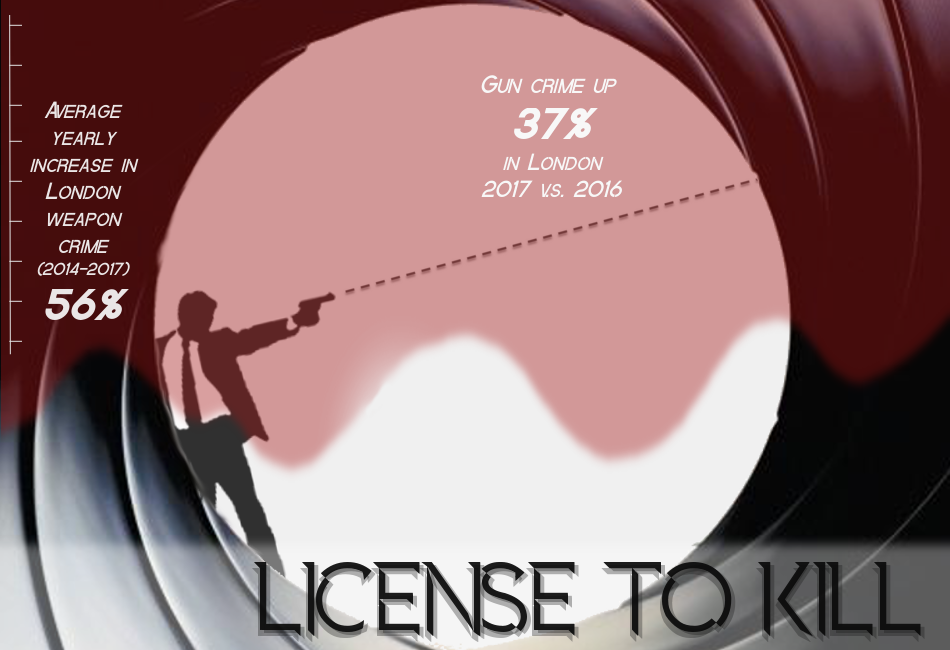
\includegraphics[width=\linewidth]{images/BondInfographic.png}
  	\end{figure}
	
\vspace{3em}

\begin{changemargin}{-3em}{-5em}
\sectionbox{\textsc{\color{electro-blue} \vspace{-1em} \hspace{5em} \section{Assumptions and Limitations} }}
\end{changemargin}
\vspace{1em}
Most assumptions are discussed throughout the code as and when they were made during the course of the project, via comments shown in the \hyperref[sec:8-0]{\color{electro-blue-dark}appendices}.
\linebreak \linebreak
In terms of limitations, main points to note include:
\vspace{1em}
\begin{itemize} % Starts unordered (bullet point) list
	\item Disregarding crime types that are not gang-related.
	\item Limiting the scope in terms of time period to homogenise many sources of data.
	\item Large amount of data slowing down visualisation.
	\item Exploratory tool rather than final analysis.

\pagebreak

\begin{changemargin}{-3em}{-5em}
\sectionbox{\textsc{\color{electro-blue} \vspace{-1em} \hspace{5em} \section{Appendices} }}
\end{changemargin}
\label{sec:8-0}
	\vspace{1em}
	
	\begin{changemargin}{-1em}{-5em}
	\subsectionbox{\textsc{\color{electro-blue} \vspace{-1em} \hspace{15em} \subsection{SQL Cleanse} }}
	\label{sec:8-1}
	\end{changemargin}
	\begin{changemargin}{0.5em}{-5em}
	\inputminted[linenos,breaklines,fontsize=\small]{sql}{Cleanse.sql}
	\end{changemargin}
	
	\pagebreak
	\begin{changemargin}{-1em}{-5em}
	\subsectionbox{\textsc{\color{electro-blue} \vspace{-1em} \hspace{15em} \subsection{Alteryx Cleanse} }}
	\end{changemargin}
	\label{sec:8-2}
	\begin{figure}[h!]
		\centering
		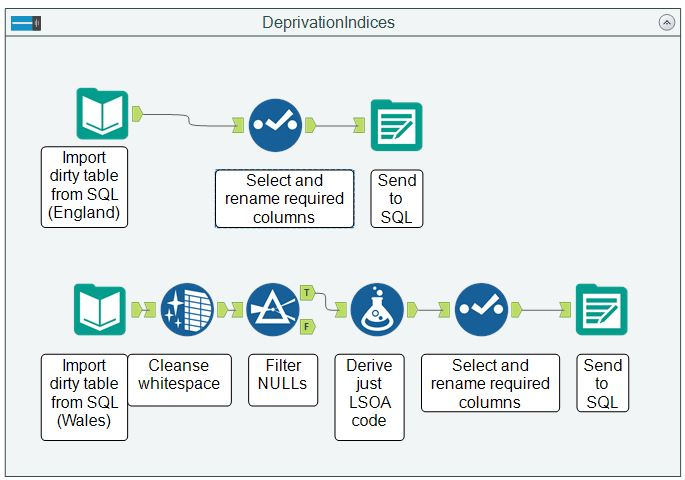
\includegraphics[width=0.8\linewidth]{images/Alteryx_Deprivation.JPG}
  	\end{figure}
  	\begin{figure}[h!]
  		\centering
		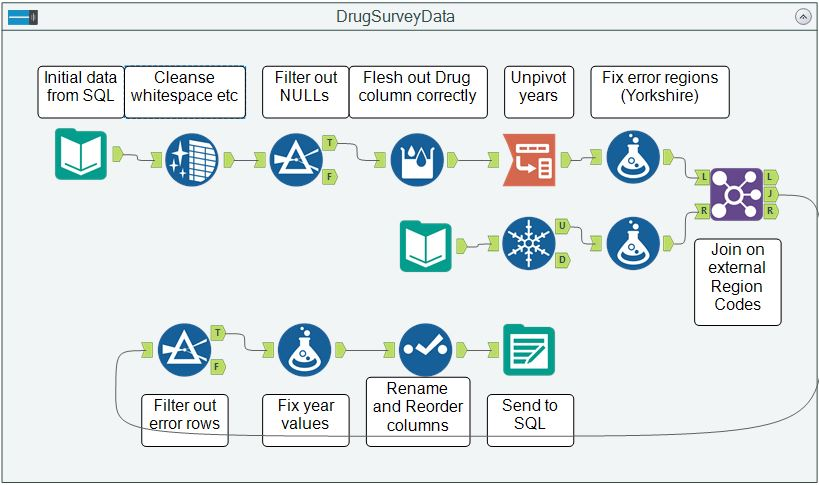
\includegraphics[width=0.8\linewidth]{images/Alteryx_DrugSurvey.JPG}
  	\end{figure}
  	\begin{figure}
  		\begin{subfigure}[t]{0.5\linewidth}
  			\centering
			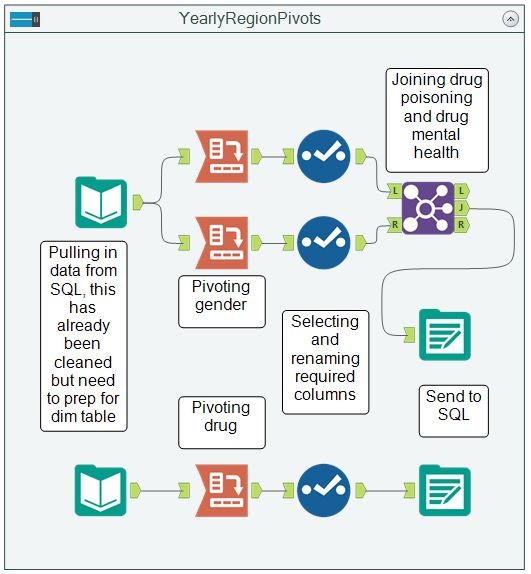
\includegraphics[width=\linewidth]{images/Alteryx_YearlyRegion.JPG}
		\end{subfigure}
		\begin{subfigure}[t]{0.5\linewidth}
  			\centering
			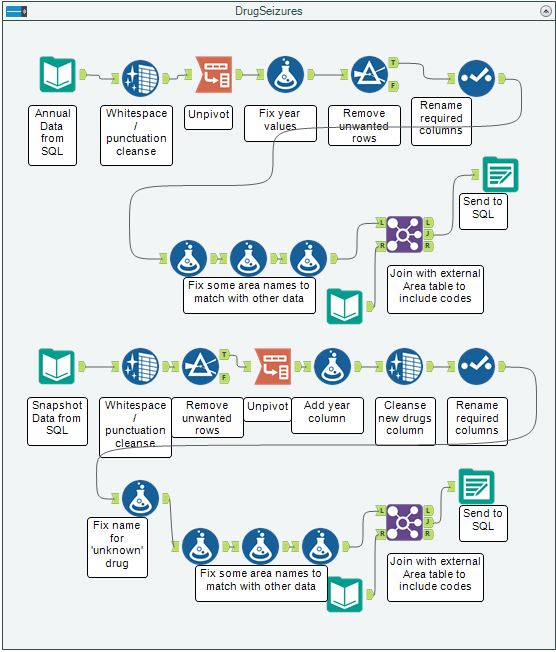
\includegraphics[width=\linewidth]{images/Alteryx_DrugSeizures.JPG}
		\end{subfigure}
  	\end{figure}
  	\begin{figure}
  		\begin{subfigure}[b]{0.5\linewidth}
  			\centering
			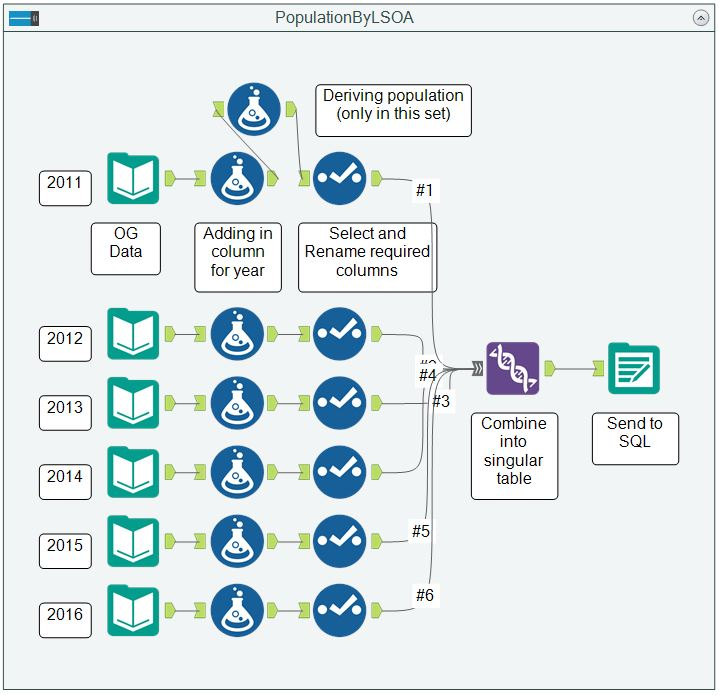
\includegraphics[width=\linewidth]{images/Alteryx_PopulationLSOA.JPG}
		\end{subfigure}
		\begin{subfigure}[b]{0.5\linewidth}
  			\centering
			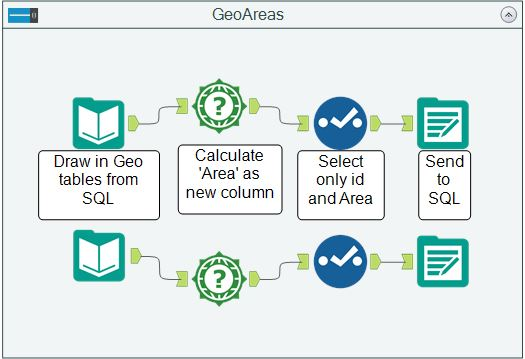
\includegraphics[width=\linewidth]{images/Alteryx_GeoAreas.JPG}
		\end{subfigure}
  	\end{figure}
  	\begin{figure}[h!]
		\centering
		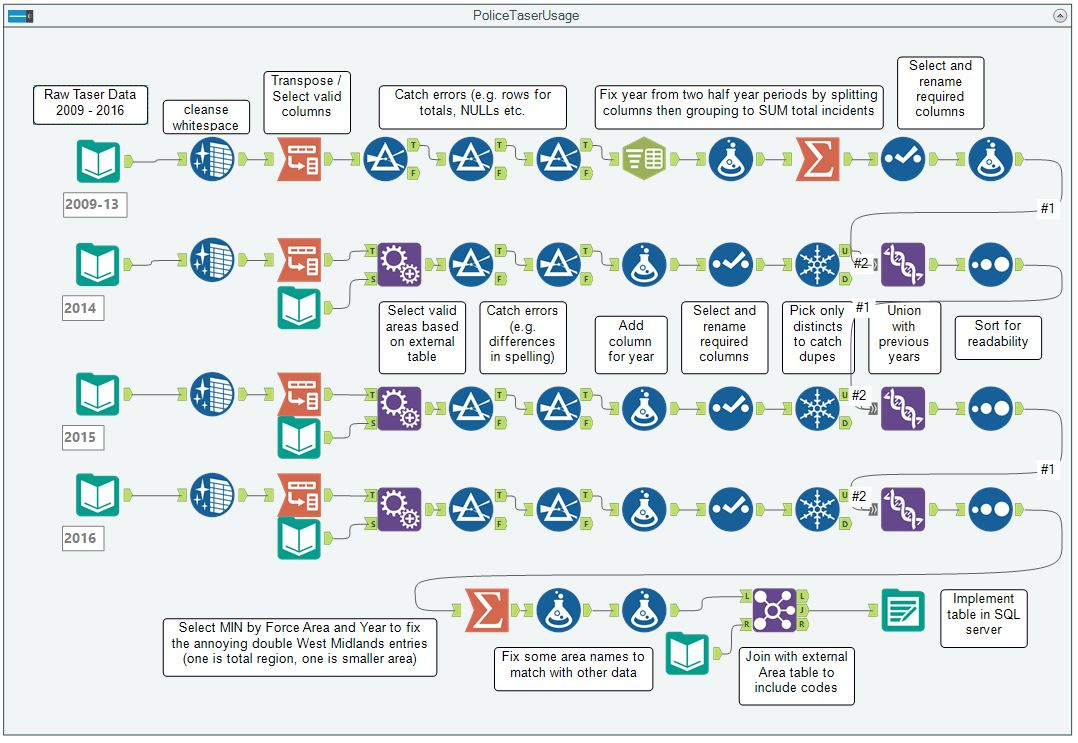
\includegraphics[width=\linewidth]{images/Alteryx_Taser.JPG}
  	\end{figure}
  	\begin{figure}[h!]
  		\centering
		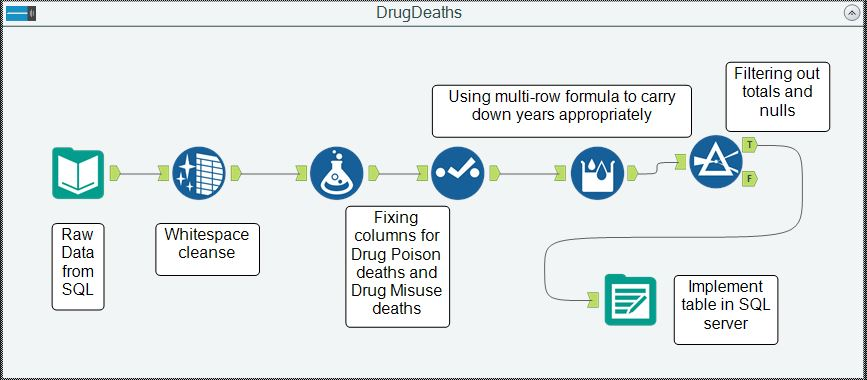
\includegraphics[width=\linewidth]{images/Alteryx_DrugDeaths.JPG}
  	\end{figure}
  	\begin{figure}[h!]
		\centering
		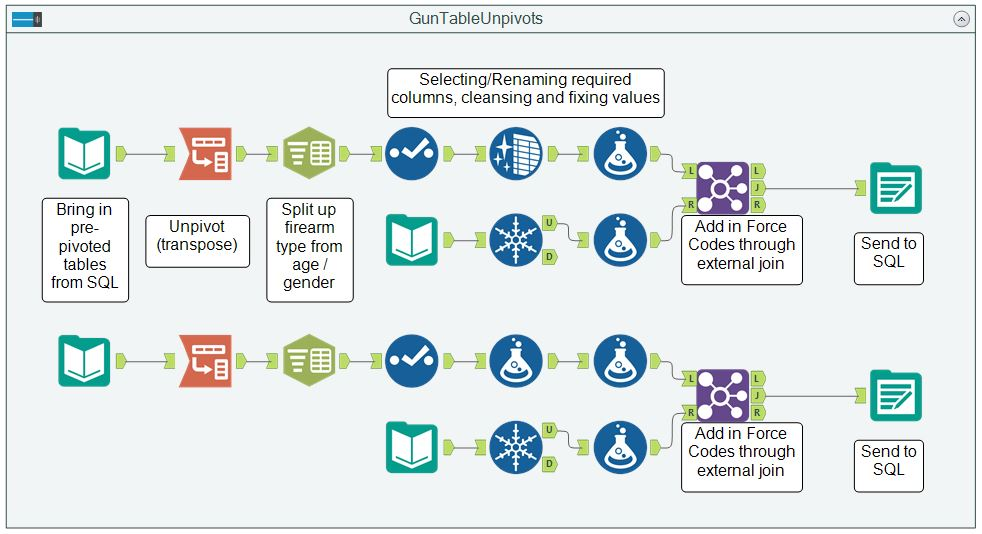
\includegraphics[width=\linewidth]{images/Alteryx_GunTable.JPG}
  	\end{figure}
  	\begin{figure}[h!]
  		\centering
		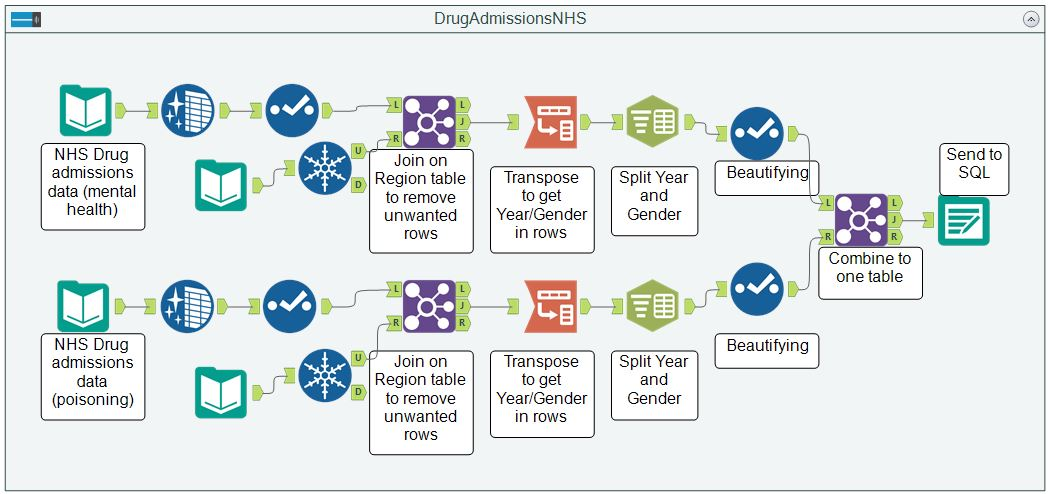
\includegraphics[width=\linewidth]{images/Alteryx_DrugNHS.JPG}
  	\end{figure}
  	\clearpage
  	
  	\begin{changemargin}{-1em}{-5em}
	\subsectionbox{\textsc{\color{electro-blue} \vspace{-1em} \hspace{15em} \subsection{SQL Modelling} }}
	\label{sec:8-3}
	\end{changemargin}
	\begin{changemargin}{0.5em}{-5em}
	\inputminted[linenos,breaklines,fontsize=\small]{sql}{Model.sql}
	\end{changemargin}
	
	\pagebreak
	\begin{changemargin}{-1em}{-5em}
	\subsectionbox{\textsc{\color{electro-blue} \vspace{-1em} \hspace{15em} \subsection{Dimensional Model} }}
	\label{sec:8-4}
	\end{changemargin}
	\begin{figure}[h!]
  		\centering
		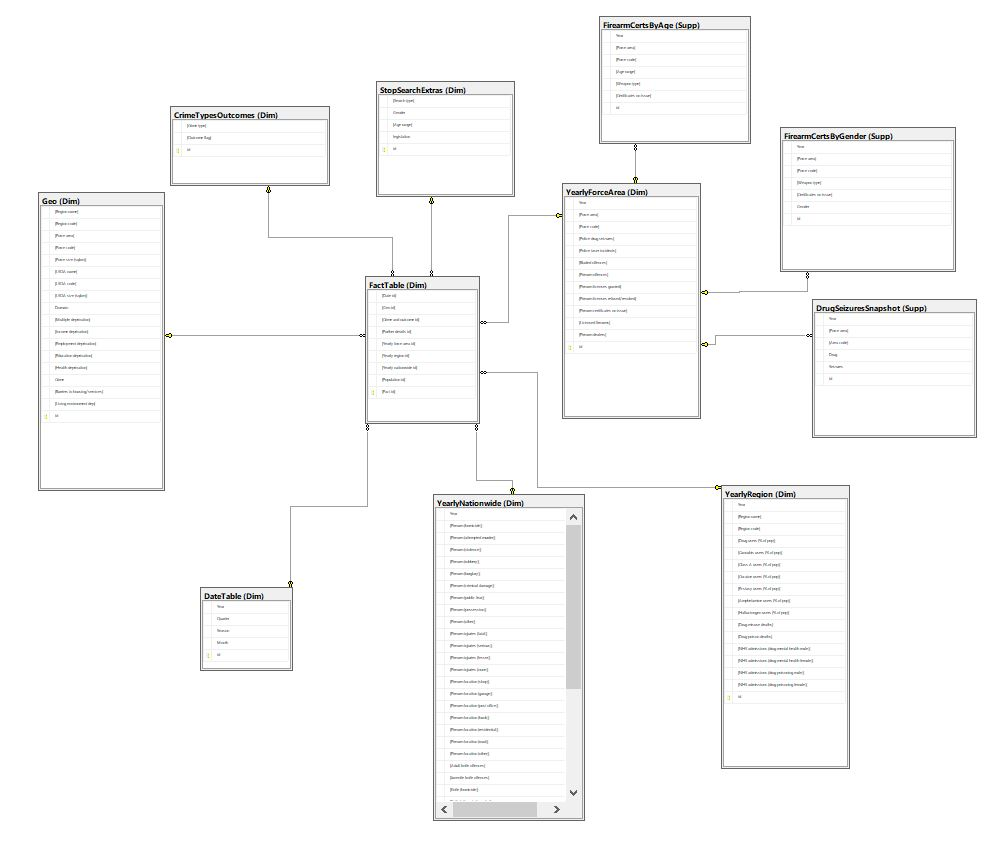
\includegraphics[width=\linewidth]{images/DimModel.JPG}
  	\end{figure}
  	\clearpage

\end{document}
